\appendix   

 \section{Enrichment Pipeline}
  \label{appdx:enrichment}
 
 \begin{figure}[H]
     \centering
     \vspace{-0.5cm}
     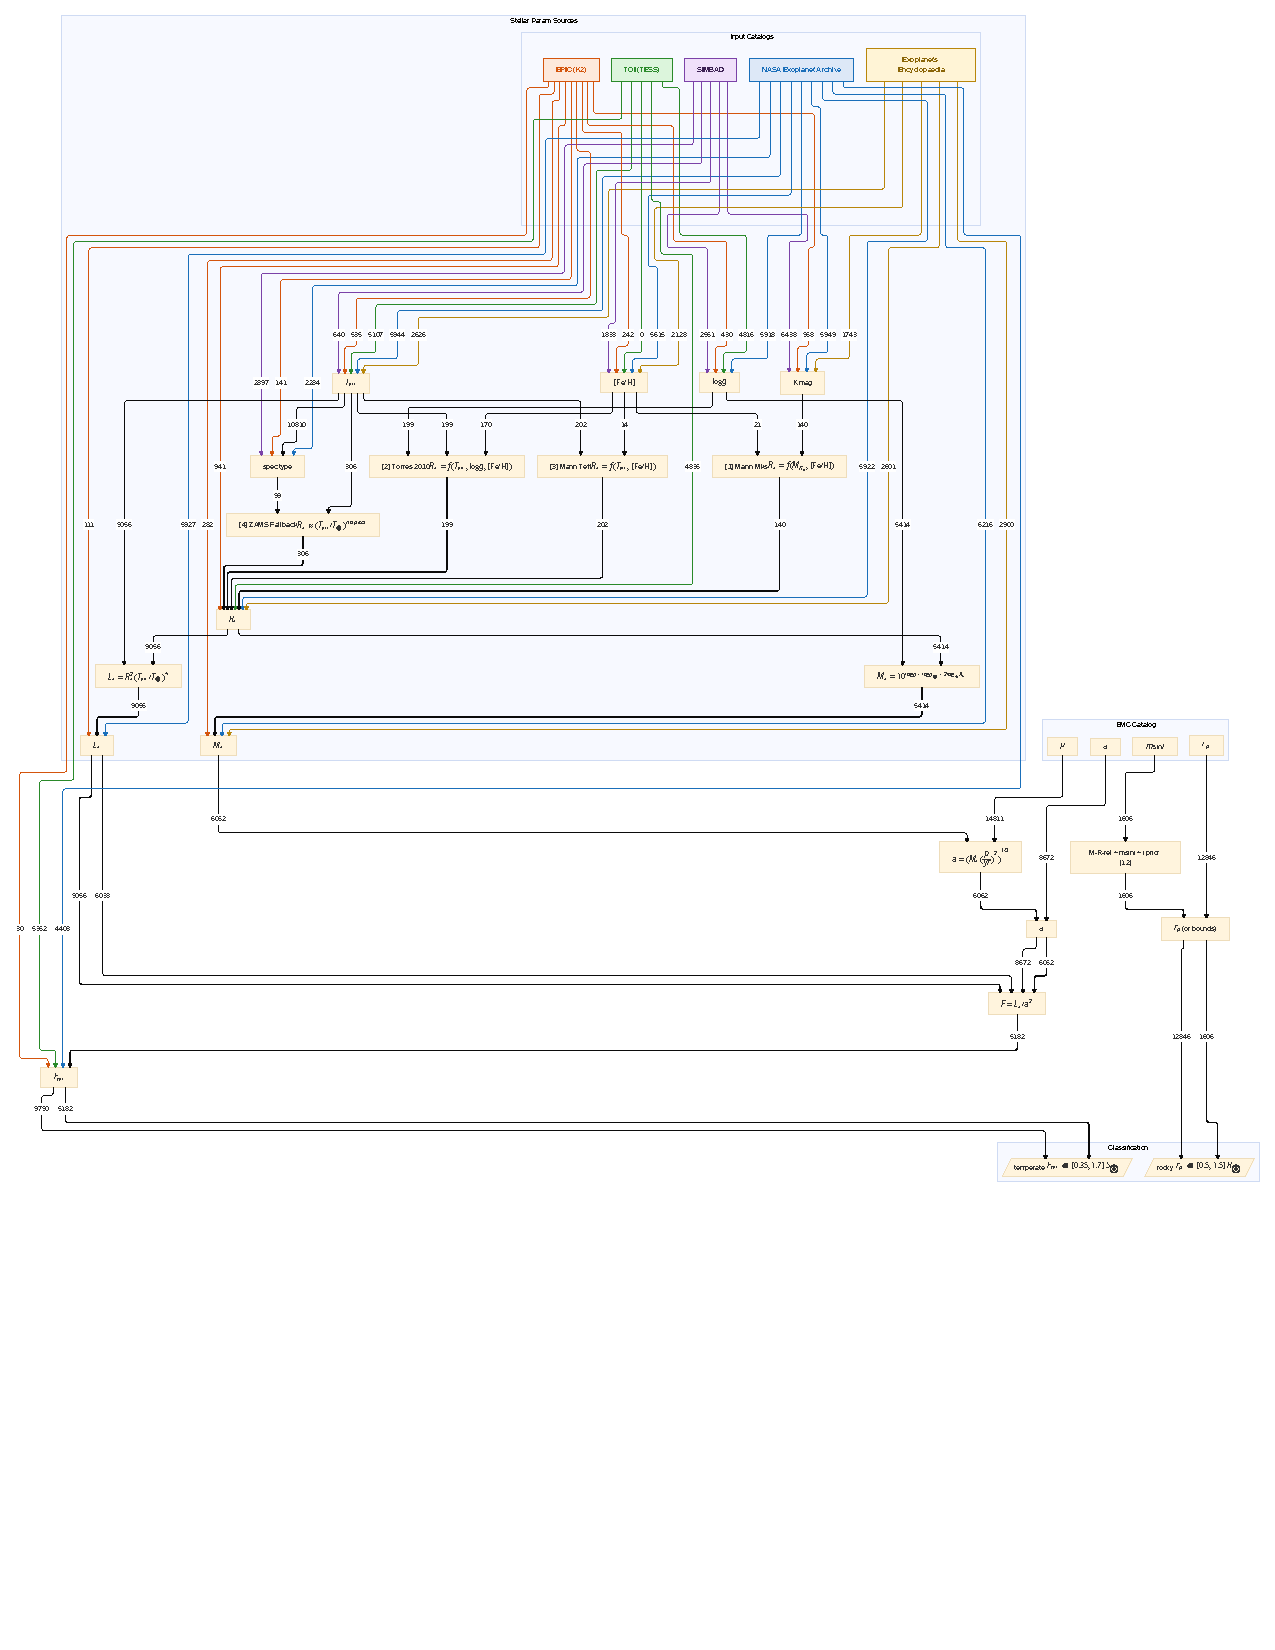
\includegraphics[width=0.9\linewidth]{figures/enrichment_pipeline_flowchart.pdf}
     \vspace{-4cm}
     \caption{The flowchart illustrates the priority-ordered data retrieval hierarchy from input sources and the subsequent empirical or  physical derivation pathways used to determine stellar parameters and orbital/planetary quantities. Solid arrows represent directly retrieved catalog values, while dashed arrows denote computed properties, with labels indicating the exact number of planet-rows processed through each transition.}
     \label{fig:enrichment_mermaid}
 \end{figure}


\section{Planet distribution without parameter computations}
\label{appddx:nocomp}
\begin{figure}[H]
    \centering
    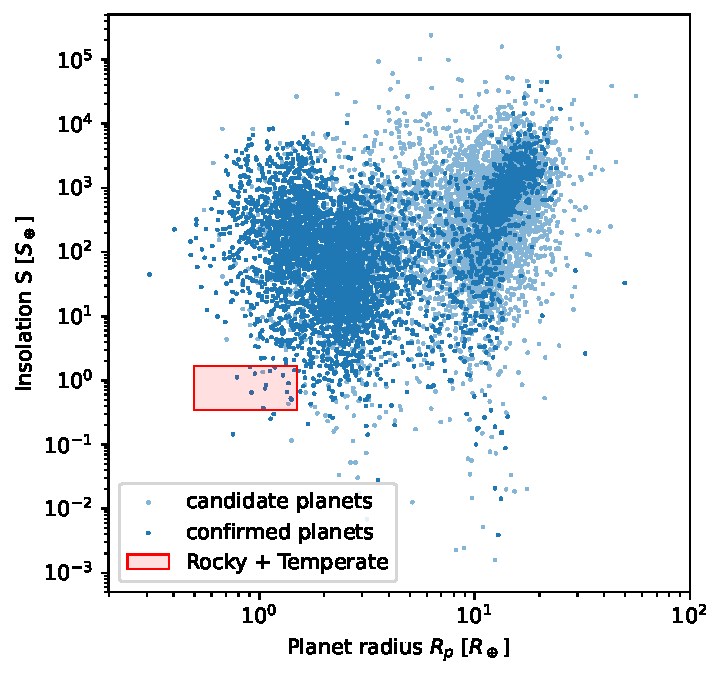
\includegraphics[width=0.72\textwidth]{figures/radius_insolation_distribution_uncomputed.pdf}
    \caption{Distribution of the enriched Exo-MerCat exoplanet population in terms of planet-radius insolation (contains no parameter computations). Confirmed planets are drawn in the darker shade and unconfirmed candidates in the lighter shade. The red rectangle marks the rocky-and-temperate selection region adopted in this work, spanning a radius of $0.5$--$1.5\,R_\oplus$ and an incident stellar flux of $0.35$--$1.7\,S_\oplus$.}
    \label{fig:pop_distr_nocomp}
\end{figure}

\section{Population by Host Spectral Category}
\label{appdx:spectral_category}

\Cref{fig:pop_heatmap_spectral} splits the planet-radius--insolation density of \cref{fig:pop_heatmap} by the spectral category assigned to the host star by the enrichment pipeline. As expected from the broader field, Sun-like hosts dominate the overall Exo-MerCat population. In the distance-limited HPICxLIFEcat crossmatch, however, the low- and very-low-luminosity categories carry a markedly larger share of the sample ($\sim$35\% of the crossmatched planets versus $\sim$12\% of the full catalog), reflecting the abundance of cool, low-mass stars in the immediate solar neighborhood that dominates the LIFE target list.

\begin{figure}[H]
    \centering
        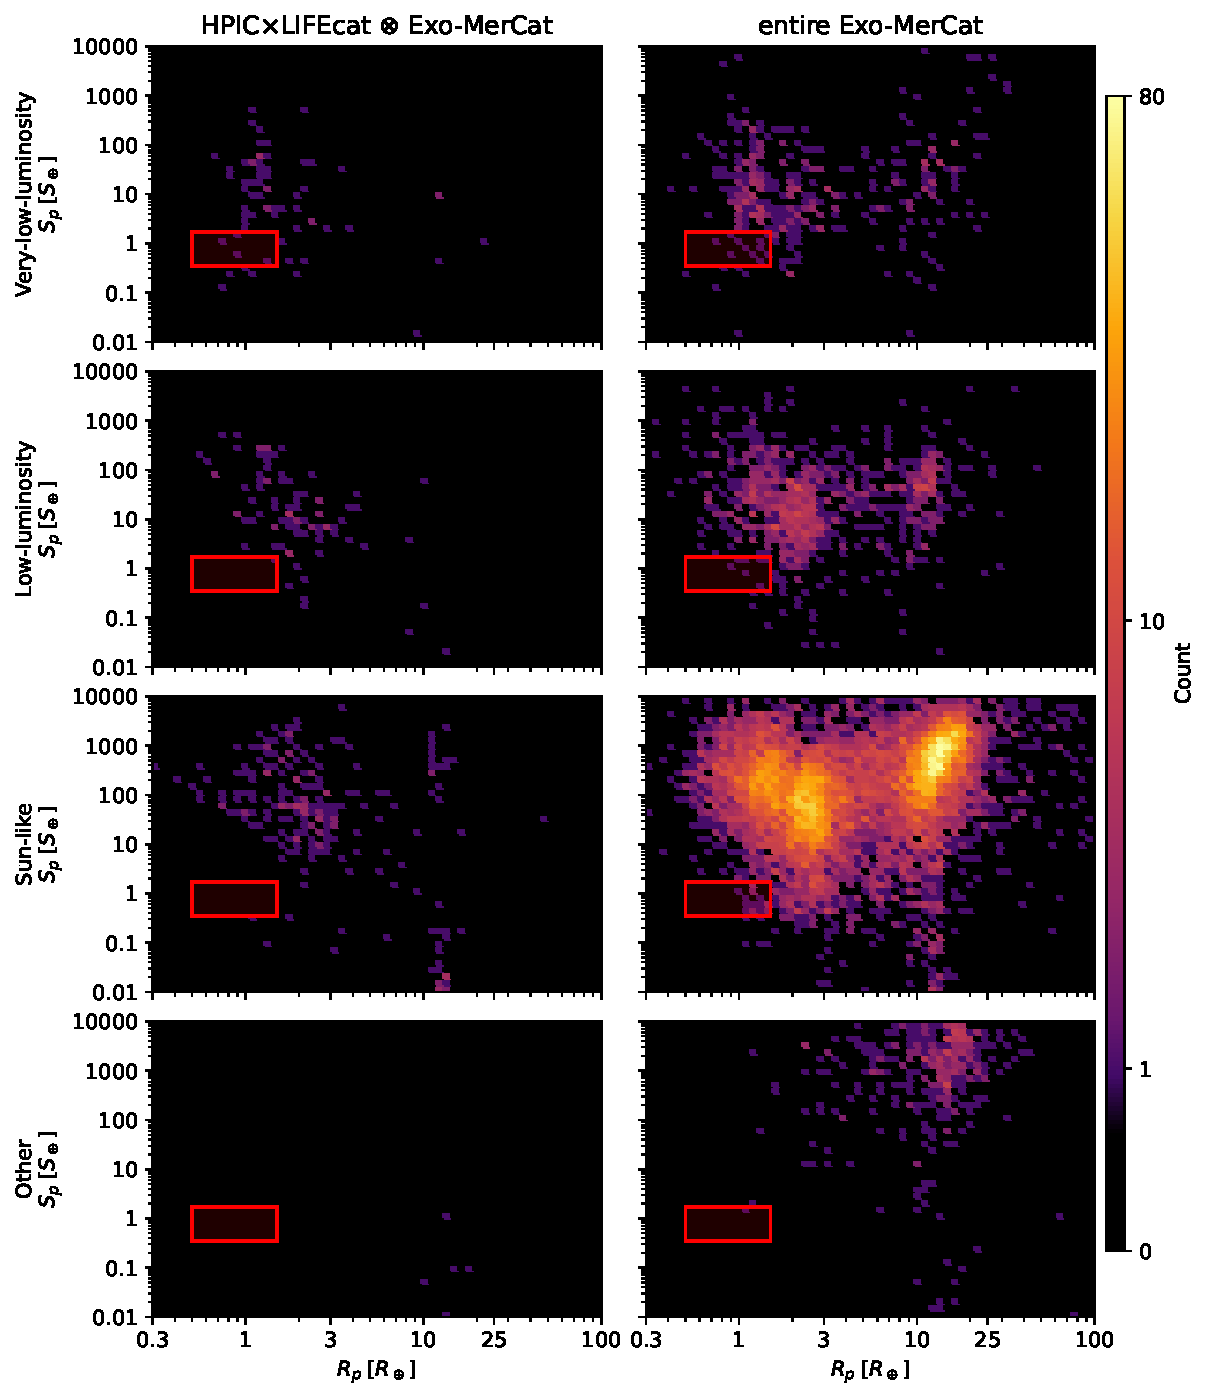
\includegraphics[width=0.9\linewidth]{figures/radius_insolation_heatmap_by_spectral_category.pdf}
    \caption{Two-dimensional number density of the exoplanet population in the planet-radius--insolation plane (as in \cref{fig:pop_heatmap}), split by the spectral category of the host star. The four rows correspond to the host categories assigned by the enrichment pipeline (Very-low-luminosity, Low-luminosity, Sun-like, and Other); the left column is the distance-limited HPIC$\times$LIFEcat sample crossmatched with Exo-MerCat and the right column the entire Exo-MerCat catalog. Both axes are logarithmic and the color encodes the number of planets per bin on a logarithmic scale, shared across all panels. The red rectangle marks the rocky-and-temperate selection region ($0.5$--$1.5\,R_\oplus$, $0.35$--$1.7\,S_\oplus$). Planet radii and insolations are those provided by the enrichment pipeline.}
    \label{fig:pop_heatmap_spectral}
\end{figure}

\section{Rocky, Temperate Planet Candidate Tables}
\label{appdx:rocky_temp_tables}

\Cref{tab:rocky_temp_table} lists the rocky, temperate planet candidates in the distance-limited HPIC$\times$LIFEcat sample crossmatched with Exo-MerCat (the same population as the top panel of \cref{fig:rocky_temp_yield}); \cref{tab:rocky_temp_table_full} lists the same selection applied to the entire enriched Exo-MerCat catalog (the bottom panel of \cref{fig:rocky_temp_yield}). 

\begin{landscape}
\centering
\input{figures/rocky_temperate_candidates_table.tex}
\end{landscape}

\begin{landscape}
\centering
\begin{longtblr}[
  caption = {Rocky, temperate planet candidates in Exo-MerCat (see \cref{fig:rocky_temp_yield})},
  label = {tab:rocky_temp_table_full},
]{colspec = {Q[l,wd=3.5cm] l l l l Q[l,wd=3cm] c}, font=\footnotesize, rowsep=1pt, row{1} = {font=\bfseries\footnotesize}, rowhead=1}
\hline\hline
Planet & Insolation Flux [\si{\Searth}] & Radius [\si{\Rearth}] & Mass [\si{\Mearth}] & Distance [\si{\parsec}] & Semi-major Axis [\si{\astronomicalunit}] & Spectral Type \\
\hline
\SetCell[c=7]{c}{\textbf{Confirmed}} \\
\hline
L 372-58 c & \num{1.40(20)} & \num{1.194(47)}\textsuperscript{c} & \num{1.81(13:11)} & \num{3.67278(89:90)} & \num{0.0350(10)} & M5.5 \\
L 372-58 d & \num{0.60(10)} & \num{1.149(76)}\textsuperscript{c} & \num{1.67(17:21)} & \num{3.67278(89:90)} & \num{0.0540(10)} & M5.5 \\
G 32-5 b & \num{1.62(13:11)} & \num{0.904(37:34)} & \num{0.71(12)} & \num{12.210(13)} & \num{0.06700(50:60)} & M3.0 \\
TRAPPIST-1 d & \num{1.115(43)} & \num{0.7880(110:100)} & \num{0.388(12)} & \num{12.430(19)} & \num{0.0223} & M8.0 \\
TRAPPIST-1 e & \num{0.646(25)} & \num{0.920(13:12)} & \num{0.692(22)} & \num{12.430(19)} & \num{0.0293} & M8.0 \\
TRAPPIST-1 f & \num{0.373(15:14)} & \num{1.045(13:12)} & \num{1.039(31)} & \num{12.430(19)} & \num{0.0385} & M8.0 \\
TOI-700 d & \num{0.850(90:100)} & \num{1.073(59:54)} & \num{2.42} & \num{31.127(21)} & \num{0.1633(27)} & M2.5 \\
TOI-700 e & \num{1.27(13:15)} & \num{0.953(89:75)} & \textemdash & \num{31.127(21)} & \num{0.1340(22)} & M2.5 \\
LP 890-9 c & \num{0.906(26)} & \num{1.367(55:39)} & \num{25(25)} & \num{32.430(70)} & \num{0.03984(22)} & M6 \\
K2-3 d & \num{1.44(14)} & \num{1.458(56:51)} & \num{2.20} & \num{44.07(11)} & \num{0.2014(34:33)} & M \\
LP 759-72 e & \num{1.20(20)} & \num{1.29(13)} & \textemdash & \num{66.43(20)} & \num{0.1060(90:130)} & \textemdash \\
Kepler-1649 A c & \num{0.750(32:302)} & \num{1.06(15:10)} & \textemdash & \num{92.19(55:54)} & \num{0.0649} & \textemdash \\
Kepler-1512 A b & \num{1.60(44:51)} & \num{1.180(70:110)} & \textemdash & \num{162.0(58:159)} & \num{0.13693(52)} & \textemdash \\
Kepler-438 b & \num{1.40(67:77)} & \num{1.12(16:17)} & \textemdash & \num{195.9(47)} & \num{0.166(51:42)} & \textemdash \\
Kepler-1229 A b & \num{0.524(54:50)} & \num{1.40(11:13)} & \num{2.54} & \num{265.5(34:33)} & \num{0.3006(69:91)} & M0 \\
Kepler-62 f & \num{0.500} & \num{1.412(67)} & \num{35.0} & \num{300.9(12)} & \num{0.7180(70)} & K2 \\
Kepler-442 b & \num{0.66(23:41)} & \num{1.35(18:11)} & \textemdash & \num{366.0(28:27)} & \num{0.409(209:60)} & \textemdash \\
\hline
\SetCell[c=7]{c}{\textbf{Uncertain}} \\
\hline
Proxima Centauri b & \num{0.641(65)} & \num{1.36(34)}\textsuperscript{c} & \num{1.055(55)}\textsuperscript{b} & \num{1.30119(34:35)} & \num{0.04848(29)} & M5.5 \\
Ross 128 b & \num{1.38} & \num{1.55(45)}\textsuperscript{c} & \num{1.40(21)}\textsuperscript{b} & \num{3.37454(80)} & \num{0.0496(17)} & M4 \\
Teegarden's Star b & \num{1.080(80)} & \num{1.42(37)}\textsuperscript{c} & \num{1.16(12:11)}\textsuperscript{b} & \num{3.8308(40)} & \num{0.02590(80:90)} & M7.0 \\
Teegarden's Star c & \num{0.350(20)} & \num{1.36(33)}\textsuperscript{c} & \num{1.05(14)}\textsuperscript{b} & \num{3.8308(40)} & \num{0.0443(14:15)} & M7.0 \\
G 158-27 b & \num{0.670(39)} & \num{1.37(34)}\textsuperscript{c} & \num{1.08(13)}\textsuperscript{b} & \num{4.8487(30)} & \num{0.0457(12)} & M5.5 \\
BD-17 588 A d & \num{1.00(45)}\textsuperscript{a} & \num{2.21(75)}\textsuperscript{c} & \num{2.721(75)}\textsuperscript{b} & \num{6.90} & \num{0.090(20)} & M3.5 \\
HD 156384 C e\textsuperscript{d} & \num{0.302(60)}\textsuperscript{a} & \num{2.20(75)}\textsuperscript{c} & \num{2.7(16:14)}\textsuperscript{b} & \num{7.2440(49:48)} & \num{0.213(20)} & M1.5 \\
HD 156384 C f\textsuperscript{d} & \num{0.56(13:11)}\textsuperscript{a} & \num{2.12(72)}\textsuperscript{c} & \num{2.5(13)}\textsuperscript{b} & \num{7.2440(49:48)} & \num{0.156(14:17)} & M1.5 \\
G 192-13 b & \num{0.910(90)} & \num{2.00(68)}\textsuperscript{c} & \num{2.30(40)}\textsuperscript{b} & \num{7.7227(48)} & \num{0.09673(80)} & M4 \\
Wolf 1069 b & \num{0.652(29:27)} & \num{1.48(40)}\textsuperscript{c} & \num{1.26(21)}\textsuperscript{b} & \num{9.5834(48)} & \num{0.0672(14)} & M5.0 \\
G 261-6 b & \num{1.80(12:11)} & \num{1.54(44)}\textsuperscript{c} & \num{1.37(23)}\textsuperscript{b} & \num{10.6267(63)} & \num{0.02971(87:93)} & M5.5 \\
L 291-115 b\textsuperscript{d} & \num{0.332(23)}\textsuperscript{a} & \num{0.79(17)} & \textemdash & \num{14.6058(61)} & \num{0.0699(14)}\textsuperscript{a} & M5 \\
HD 6660 .01\textsuperscript{d} & \num{1.39} & \num{2.24(92)} & \textemdash & \num{20.527(29)} & \num{1.87(14)}\textsuperscript{a} & K4 \\
TOI-4336 .01 & \num{1.69} & \num{2.05(76)} & \textemdash & \num{22.546(38)} & \num{0.0850(17)}\textsuperscript{a} & M3.5 \\
CD-34 1169 .01\textsuperscript{d} & \num{0.431} & \num{1.37(77)} & \textemdash & \num{25.143(30)} & \num{1.176(24)}\textsuperscript{a} & M \\
LP 873-20 b\textsuperscript{d} & \num{1.54}\textsuperscript{a} & \num{1.16(25)} & \textemdash & \num{26.075(22)} & \textemdash & \textemdash \\
2MASS J06034353-8127303 .01\textsuperscript{d} & \num{1.35} & \num{1.04(17)} & \textemdash & \num{26.741(63)} & \num{0.0258(13)}\textsuperscript{a} & \textemdash \\
G 125-49 b & \num{1.68(17:37)} & \num{1.65(22:20)} & \textemdash & \num{32.027(45)} & \num{0.05722(44)} & M3.5 \\
LSPM J1957+5658 .01\textsuperscript{d} & \num{0.382} & \num{1.81(66)} & \textemdash & \num{32.609(44)} & \textemdash & M4.0 \\
PM J13119+6550 d & \num{1.30(30:20)} & \num{1.70(58)}\textsuperscript{c} & \num{3.7(10:11)}\textsuperscript{b} & \num{36.012(30)} & \num{0.1513(24)} & M2 \\
MCC 189 .01\textsuperscript{d} & \num{0.406} & \num{1.74(84)} & \textemdash & \num{39.889(31)} & \num{1.51(16)}\textsuperscript{a} & M0 \\
LSPM J1902+7525 c & \num{1.84(17)} & \num{1.334(78)} & \num{7.40} & \num{41.918(50)} & \num{0.1370(60)} & M2.5 \\
TOI-715 b & \num{0.67(15:20)} & \num{1.550(64)} & \num{3.02} & \num{42.405(86:85)} & \num{0.0830(27)} & M4 \\
LP 425-186 .01\textsuperscript{d} & \num{35(32:39)}\textsuperscript{a} & \num{1.26(39:87)} & \textemdash & \num{42.89(18)} & \num{0.0117(23:40)}\textsuperscript{a} & \textemdash \\
HD 137010 b & \num{0.300(68:204)}\textsuperscript{a} & \num{1.060(61)} & \textemdash & \num{44.860(30)} & \num{0.88(30:10)} & K3.5 \\
2MASS J05021345+1442367 .01\textsuperscript{d} & \num{0.60(22)}\textsuperscript{a} & \num{1.233(116:94)} & \textemdash & \num{45.99(72)} & \num{0.05061(52)}\textsuperscript{a} & M4 \\
2MASS J05021345+1442367 .02\textsuperscript{d} & \num{0.268(98)}\textsuperscript{a} & \num{0.505(88:84)} & \textemdash & \num{45.99(72)} & \num{0.07552(77)}\textsuperscript{a} & M4 \\
2MASS J14441864+8426548 .01\textsuperscript{d} & \num{0.644} & \num{1.64(90)} & \textemdash & \num{61.761(85)} & \num{0.2979(62)}\textsuperscript{a} & \textemdash \\
CD-64 238 .01\textsuperscript{d} & \num{0.836} & \num{2.09(66)} & \textemdash & \num{62.51(14)} & \num{1.52(32)}\textsuperscript{a} & \textemdash \\
Kepler-138 e & \num{1.73(12)} & \num{0.82(15)}\textsuperscript{c} & \num{0.429(191:95)} & \num{66.86(11)} & \num{0.1803(14)} & M1 \\
LP 613-39 b & \num{1.36(159:81)} & \num{2.25(53:96)} & \textemdash & \num{82.96(37)} & \num{0.091(13:16)} & M2.5 \\
HD 87794 .01\textsuperscript{d} & \num{0.467} & \num{2.3(13)} & \textemdash & \num{83.6} & \num{1.58} & G3 \\
BD+83 461 .01\textsuperscript{d} & \num{0.857} & \num{1.63(67)} & \textemdash & \num{99.90(25)} & \textemdash & G0 \\
BD+42 1620 b\textsuperscript{d} & \num{0.653} & \num{2.8(15)} & \textemdash & \num{110} & \num{1.62} & G0 \\
TYC 8897-1221-1 .01\textsuperscript{d} & \num{0.379} & \num{2.6(11)} & \textemdash & \num{159.05(50)} & \num{1.63(10)}\textsuperscript{a} & \textemdash \\
K2-296 b & \num{1.71(43:51)}\textsuperscript{a} & \num{1.87(20:45)} & \textemdash & \num{159.3(14)} & \num{0.1346(123:53)}\textsuperscript{a} & \textemdash \\
Kepler-296 A e & \num{1.41(25:21)} & \num{1.52(27:25)} & \textemdash & \num{167(21:20)} & \num{0.169(29:28)} & M2 \\
Kepler-296 A f & \num{0.62(11:10)} & \num{1.80(31:30)} & \textemdash & \num{167(21:20)} & \num{0.255(43:42)} & M2 \\
Kepler-186 f & \num{0.30(10:15)} & \num{1.166(78)} & \textemdash & \num{177.59(77)} & \num{0.356(48)} & M1 \\
CPD-62 485 .03\textsuperscript{d} & \num{1.03} & \num{3.0(19)} & \textemdash & \num{193} & \num{1.59} & \textemdash \\
CD-61 922 .01\textsuperscript{d} & \num{1.69} & \num{3.3(22)} & \textemdash & \num{232.3(12)} & \num{1.62(11)}\textsuperscript{a} & \textemdash \\
Kepler-1652 b & \num{0.81(16:13)} & \num{1.60(18)} & \textemdash & \num{252(32:30)} & \num{0.1654(42:75)} & \textemdash \\
BD-06 3861 .01\textsuperscript{d} & \num{209(981:329)}\textsuperscript{a} & \num{2.8(65:15)} & \textemdash & \num{273.7(41:40)} & \num{0.169(34:31)}\textsuperscript{a} & F2 \\
KOI-5087 .01\textsuperscript{d} & \num{0.714}\textsuperscript{a} & \num{1.55(59:35)} & \textemdash & \num{307.13(83)} & \num{1.45} & \textemdash \\
UCAC4 665-070369 b\textsuperscript{d} & \num{0.369(70)}\textsuperscript{a} & \num{1.51(13)} & \textemdash & \num{330.9(30)} & \num{0.444(40)} & \textemdash \\
KOI-4878 b\textsuperscript{d} & \num{1.05}\textsuperscript{a} & \num{1.04(38:14)} & \textemdash & \num{349.9(11)} & \num{1.14} & G4 \\
Kepler-1505 A .02\textsuperscript{d} & \num{0.483}\textsuperscript{a} & \num{1.18(44:16)} & \textemdash & \num{359} & \num{1.20} & G0.5 \\
KOI-7179 .01\textsuperscript{d} & \num{1.30}\textsuperscript{a} & \num{1.18(49:22)} & \textemdash & \num{397.0(14)} & \num{1.08} & G2 \\
KOI-6108 .01\textsuperscript{d} & \num{0.612}\textsuperscript{a} & \num{1.07(47:16)} & \textemdash & \num{408.7(45)} & \num{1.13} & \textemdash \\
KOI-5806 .01\textsuperscript{d} & \num{1.29}\textsuperscript{a} & \num{1.26(49:13)} & \textemdash & \num{439.8(17)} & \num{0.898} & \textemdash \\
KOI-5938 .01\textsuperscript{d} & \num{1.03}\textsuperscript{a} & \num{1.66(100:22)} & \textemdash & \num{538.9(29)} & \num{1.34} & G0 \\
KOI-5948 .01\textsuperscript{d} & \num{0.580}\textsuperscript{a} & \num{1.233(549:80)} & \textemdash & \num{539.1(32)} & \num{0.996} & G5 \\
Kepler-452 b & \num{1.10(29:22)} & \num{1.63(23:20)} & \textemdash & \num{551.7(52:51)} & \num{1.046(19:15)} & G2 \\
Kepler-1126 c & \num{2.06(76:59)} & \num{1.45(18)} & \textemdash & \num{635.7(68)} & \num{0.619} & \textemdash \\
KOI-5545 .01\textsuperscript{d} & \num{0.429}\textsuperscript{a} & \num{1.081(482:69)} & \textemdash & \num{678(54)} & \num{1.25} & \textemdash \\
KOI-7235 .01\textsuperscript{d} & \num{0.752}\textsuperscript{a} & \num{1.155(381:80)} & \textemdash & \num{707(293)} & \num{0.825} & \textemdash \\
Kepler-51 e & \num{1.142(40)}\textsuperscript{a} & \num{2.09(74)}\textsuperscript{c} & \num{5.4(15)} & \num{784(14:13)} & \num{0.795(14)}\textsuperscript{a} & \textemdash \\
KOI-5068 .01\textsuperscript{d} & \num{1.69}\textsuperscript{a} & \num{1.57(52:24)} & \textemdash & \num{806.2(99)} & \num{1.01} & \textemdash \\
KOI-5819 .01\textsuperscript{d} & \num{0.483}\textsuperscript{a} & \num{1.244(415:80)} & \textemdash & \num{836(13)} & \num{0.955} & \textemdash \\
KOI-5737 .01\textsuperscript{d} & \num{0.988}\textsuperscript{a} & \num{1.32(50:13)} & \textemdash & \num{875.0(90)} & \num{1.01} & \textemdash \\
KOI-5499 .01\textsuperscript{d} & \num{1.43}\textsuperscript{a} & \num{1.19(15:11)} & \textemdash & \num{879(17)} & \num{0.419} & \textemdash \\
KOI-7223 .01\textsuperscript{d} & \num{0.570}\textsuperscript{a} & \num{1.52(38:12)} & \textemdash & \num{986(32)} & \num{0.835} & \textemdash \\
KOI-5506 .01\textsuperscript{d} & \num{0.659}\textsuperscript{a} & \num{1.61(80:13)} & \textemdash & \num{1006(15)} & \num{1.50} & \textemdash \\
KOI-6425 .01\textsuperscript{d} & \num{0.677}\textsuperscript{a} & \num{1.46(57:19)} & \textemdash & \num{1120(17)} & \num{1.22} & \textemdash \\
KOI-4986 .01\textsuperscript{d} & \num{0.468}\textsuperscript{a} & \num{1.480(471:80)} & \textemdash & \num{1323(515)} & \num{1.06} & \textemdash \\
KOI-6151 .01\textsuperscript{d} & \num{0.466}\textsuperscript{a} & \num{1.356(471:90)} & \textemdash & \num{1547(34)} & \num{1.04} & \textemdash \\
\hline\hline
\end{longtblr}


\end{landscape}
